% $Id$

GnuPG, also commonly known as GPG, is a free implementation of the
OpenPGP set of cryptography operations from the GNU Project, commonly
available as standard on open source systems such as GNU/Linux and BSD 
distributions.


\subsection{How OpenPGP (and hence GPG) Works}

The OpenPGP set of cryptographic functions include digitally signing and
encrypting a transmission. To perform such tasks, asymmetric key pairs,
commonly referred to as public private keys, are required. These keys
contain user identities (names and email addresses), and are secured 
with a pass-phrase, and are generated by individual users during the 
bootstrapping phase.


Once a user has created a key pair, they must build a Web of Trust 
(WoT), consisting of the public keys of other, trusted users.
Transmissions are encrypted using the public key of the recipient and
the key pair of the sender, ensuring only the sender and recipient are
able to decrypt and/or verify the transmission.


While this system is cryptographically secure, it is only as strong as
the weakest link, which is the human element. Unless 
good password/pass phrase practices\footnote{Eg: periodic changes, use 
of alphanumeric and non alphanumeric characters, not sharing passwords 
or noting passwords down on paper} are employed, a key-pair is only as 
strong as the pass-phrase associated with the keys and how the owner of 
the keys maintains the pass-phrase.


Additionally, a secure method of distributing public keys is required to
ensure a malicious individual does not attempt to alter a public key in
an effort to intercept encrypted communications

\subsubsection{The Web Of Trust}

\begin{figure}[p]

\label{fig:wot}

\begin{center}

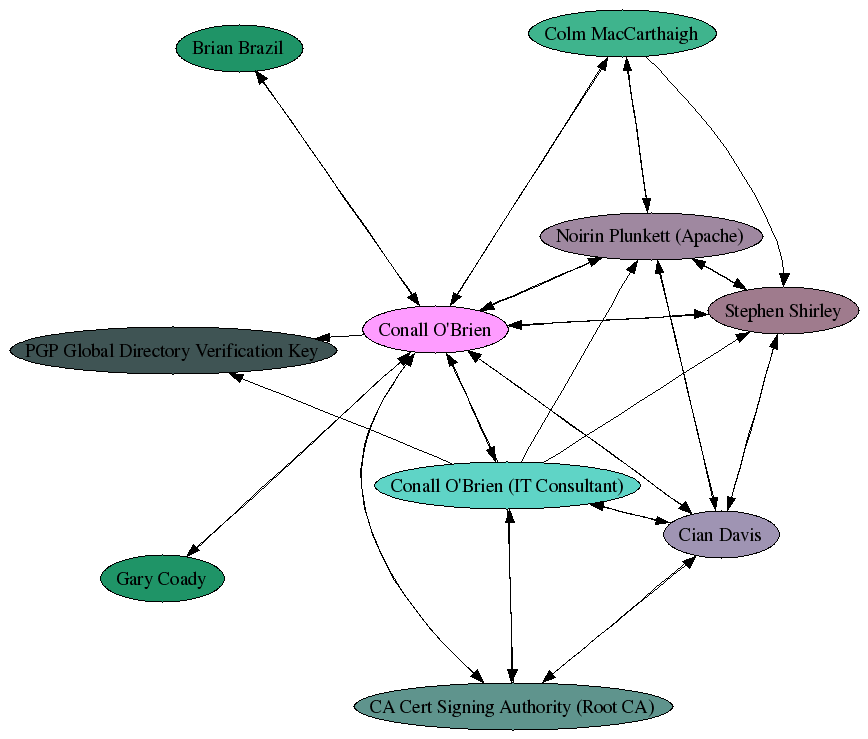
\includegraphics[bb= 0 0 868 739,scale=0.5]{include/EE7DC74E.png}

\end{center}

\caption{Graphical Representation of the WoT for OpenPGP Key 0xEE7DC74E}

\end{figure}

\pagebreak

\subsection{Cryptography Algorithms}

=== Rewrite ===


GPG encrypts messages using asymmetric key-pairs individually generated
by GPG users. The resulting public keys can be exchanged with other
users in a variety of ways, such as Internet key servers. They must
always be exchanged carefully to prevent identity spoofing by
corrupting public key 'owner' identity correspondences. It is
also possible to add a cryptographic digital signature to a message, so
the message integrity and sender can be verified, if a particular
correspondence relied upon has not been corrupted.

GPG does not use patented or otherwise restricted software or
algorithms, including the IDEA encryption algorithm which has been
present in PGP almost from the beginning. Instead, it uses a variety of
other, non-patented algorithms such as CAST5, Triple DES, AES, Blowfish
and Twofish. It is still possible to use IDEA in GPG by downloading a
plug-in for it, however this may require getting a license for some uses
in some countries in which IDEA is patented.

GPG is a hybrid encryption software program in that it uses a
combination of conventional symmetric-key cryptography for speed, and
public-key cryptography for ease of secure key exchange, typically by
using the recipient's public key to encrypt a session key which is only
used once. This mode of operation is part of the Open PGP standard and
has been part of PGP from its first version.

=== End rewrite ===

Further information about public private key cryptography, including key
management is available in Applied Cryptography by Bruce Sneider.
